\chapter{SSH}
SSH, or Secure Shell, is a \textbf{network protocol} that allows for
\textbf{secure communication} between two computers, which makes it a
\textit{"competitor"} of the much more used TLS protocol. It has been
introduced in 1995 by Tatu Ylönen, a Finnish computer science student,
as a response to a security incident per which the FTP credentials of 
his university were sniffed, but it has been commercialized since so
it was not open source anymore. A open source fork called OpenSSH has
been introduced in OpenBSD in 1999, and has been standardized in 2006
by the IETF in RFC 4251, referred to it as SSH-2.
\begin{boxH}
  As it is the most used version, here we will always refer to SSH-2
  (unless otherwise noted)
\end{boxH}

\section{Architecture}
From an architectural point of view, SSH is a three layer
architecture, which means it is simpler than TLS. SSH uses TCP as the
Transport Layer Protocol, but the SSH transport layer provides a nice
set of features, which are \textbf{initial connection}, \textbf{server
authentication}, \textbf{confidentiality} and \textbf{integrity} and
\textbf{key re-exchange} (RFC-4253 recommends after 1GB of data
transmitted or after 1 hour of transmission, notice that this does not
refer specifically to SSH bu to  any encrypted channel) which is
crucial for long running connections.
\begin{boxH}
  Beware that the SSH transport layer is not the same as the TCP
  transport layer, but it is a layer that is built on top of the TCP 
  transport layer, even though they have similar names.
\end{boxH}
There's also a specific protocol for \textbf{user authentication},
compulsory with SSH, and a \textbf{connection protocol} too, which
supports supports multiple connections (channels) over a single secure
channel (implemented with the transport layer protocol). This means
that SSH can act as a site-to-site VPN.
\subsection{SSH Transport Layer Protocol}
The general schema of an SSH connection is shown in figure
\ref{fig:ssh-layer-protocol}.\\
The connection is setup with TCP, by default on port 22, on which the
client initiates the connection.\\
Then the SSH version string is exchanges by both sides, which contains
the security features supported. Both sides must send a
\textbf{version string} of the following form(the pipe symbol is used
to separate the fields): 

\begin{center}
\texttt{
SSH-protoversion-softwareversion|SP|comments|CR|LF
}\\
\end{center}
SP is a space character, CR is a carriage return character and LF is a
line feed character. If the comments are omitted, the SP is also
omitted.\\
Its also used to triggers compatibility extensions and to advertise
the protocol implementation capabilities.\\
A \textbf{key exchange} follows, which includes algorithm negotiation
for the key exchange itself.\\
After this point data can be exchanged, and the connection is closed
when the data exchange is finished.\\
The termination of the TCP connection is not part of the protocol
itself, but it's performed by TCP itself.\\
\begin{figure}[H]
  \centering
  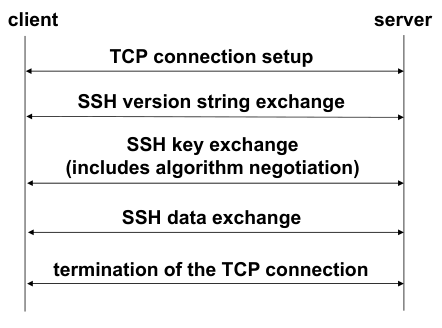
\includegraphics[width=.6\textwidth]{img/SSH layer protocol.png}
  \caption{SSH Transport Layer Protocol}
  \label{fig:ssh-layer-protocol}
\end{figure}
\subsubsection{Binary Packet Protocol}
All packets that follow the version string exchange is sent using the
Binary Packet Protocol, which is roughly the basic unit on
transmission. Every message in this kind of packet is sent as a
sequence of bytes.
\begin{figure}[h]
  \centering
  \includegraphics[width=.6\textwidth]{img/SSH bynary packet
  protocol.png}
  \caption{Binary Packet Protocol}
\end{figure}
The Binary Packet Protocol is pretty simple, it consists of:
\begin{itemize}
  \item the \textbf{length} of the \textbf{packet} (4 bytes), which
    does not include the MAC and the packet length field itself
  \item the \textbf{padding length} (1 byte), which is the length of
    the random padding field
  \item the \textbf{payload}, which may be compressed. Its size is the
    length of the packet minus the length of the length field minus 1
    (for the padding length field), up to a maximum uncompressed size
    of 32768 bytes(32KB)
  \item the \textbf{random padding}, minimum 4 bytes, up to the entire
    size of one block, and random to add confusion to the packet
  \item the \textbf{MAC}, computed over the clear text packet and the
    implicit sequence number
\end{itemize}
The first 4 fields are encrypted.

\subsubsection{Key exchange}
Another essential part of the SSH protocol is the key exchange, which 
is used to established the keys and to negotiate the algorithms to
been used.\\
One peculiarity of the SSH protocol is that the algorithms used are
selected based on directionality, which means that it is possible to
use different algorithms for the client-to-server and server-to-client
communication.\\
SSH-2 allows to select the key exchange function as well as the hash
algorithm to be used in the key derivation function. 
\begin{boxH}
  This means that the two parties have \textit{"full"} control over 
  the algorithms to be used(if supported).
\end{boxH}
  
Another interesting aspect of the protocol is that, as it was proposed
as an alternative to the Telnet protocol, it included negotiation of
the language to be used, because of the text-only nature of the 
protocol.\\
The last field of the key exchange(first key exchange packet follows)
contains an attempt to guess the agreed key exchange algorithm.\\
It contains the following fields:
\begin{itemize}
    \item SSH\_MSG\_KEXINIT
    \item cookie (16 random bytes)
    \item kex\_algorithms
      \begin{itemize}
        \item eg:diffie-hellman-group1-sha1, ecdh-sha2-OID\_of\_curve
      \end{itemize}
    \item server\_host\_key\_algorithms: used for the server authentication
      \begin{itemize}
        \item eg:ssh-rsa, ssh-dss, ecdsa-sha2-NISTP256
      \end{itemize}
    \item encryption\_algorithms\_client\_to\_server, \dots server\_to\_client
      \begin{itemize}
        \item aes-128-cbc, aes-256-ctr, aead\_aes\_128\_gcm
      \end{itemize}
    \item mac\_algorithms\_client\_to\_server, \dots server\_to\_client
      \begin{itemize}
        \item hmac-sha1, hmac-sha2-256, aead\_aes\_128\_gcm
      \end{itemize}
    \item compression\_algorithms\_client\_to\_server, \dots server\_to\_client
      \begin{itemize}
        \item none, zlib
      \end{itemize}
    \item languages\_client\_to\_server, \dots server\_to\_client
    \item first\_kex\_packet\_follows (flag)
\end{itemize}
Keep in mind that because of the negotiation of the protocols to be
used, SSH is potentially vulnerable to downgrade attacks.
\begin{boxH}
  A complete list of the supported algorithms can be found
  \href{https://www.iana.org/assignments/ssh-parameters/ssh-parameters.xhtml}{\textbf{here}}
\end{boxH}

\subsubsection{Diffie-Hellman key agreement}
This is also an \textbf{implicit authentication} of the server, due to
the fact that the server can compute the correct premaster secret
using the private key.\\
In this phase the client generates a random number $x$ and computes
$e=g^x \mod p$ and sends it to the server. The server generates a
random number $y$ and computes $f=g^y \mod p$ and sends it to the
client. At this point the key $K$ has been established. The server
computes the \textbf{exchange hash} $H$ over many fields(which makes
it basically a keyed digest): 
\begin{itemize}
  \item the client version string
  \item the server version string
  \item the client's KEXINIT message
  \item the server's KEXINIT message
  \item the shared secret $K$
  \item the exchange value $f$
  \item the exchange value $e$
  \item the host public key
\end{itemize}
and signs it with its private key to generate the signature $sigH$.\\
Those two values, together with the host public key in a raw format,
are sent to the client, which verifies the signature and computes the
same hash value. Notice that because the public key is sent in a raw 
format, the client must have a copy of the server's public key stored 
locally, and this is one of the major attack vectors of SSH.\\
Notice also that, because many algorithms need an initialization
vector, which is computed using an hash algorithm over $H$, which
makes it a keyed digest, again.


\begin{tikzpicture}[node distance=4cm, auto]
    % Define styles
    \tikzset{
        every node/.style={font=\small},
        process/.style={rectangle, draw, text centered, minimum height=1.5em, font=\small},
        data/.style={rectangle, draw, rounded corners, align=center, font=\small},
        arrow/.style={-{Latex[length=2mm]}, thick}
    }

    % Nodes for client (C) and server (S)
    \node (C) [process] {Client [C]};
    \node (S) [process, right=4cm of C] {Server [S]};

    % Client side steps
    \node (C1) [data, below=1cm of C] {Generates random number x\\$e = g^x \mod p$};
    \node (C3) [data, below=4.5cm of C1] {Verifies $s\_host\_PK$\\Computes $K = f^x \mod p = g^{xy} \mod p$\\Computes $H = HASH(...)$};
    \node (C4) [data, below=1cm of C3] {Verifies signature $sigH$};
    \node (C5) [data, below=1cm of C4] {$H$ becomes session-id};

    % Server side steps
    \node (S1) [data, below=1cm of S] {Generates random number y\\$f = g^y \mod p$};
    \node (S2) [data, below=1cm of S1] {Computes $K = e^y \mod p = g^{xy} \mod p$\\Computes $H = HASH(...)$};
    \node (S3) [data, below=1cm of S2] {Generates signature $sigH$\\Signs using private key $s\_host\_SK$};
    \node (S4) [data, below=1cm of S3] {$ex=s\_host\_PK \mid f \mid sigH$};
    \node (S5) [data, below=3cm of S4] {$H$ becomes session-id};

    % Arrows between nodes
    \draw [arrow] (C1) -- (S1) node[midway, above] {$e$};
    \draw [arrow] (S1) -- (S2);
    \draw [arrow] (S2) -- (S3);
    \draw [arrow] (S3) -- (S4);
    \draw [arrow] (S4) -- (C3) node[midway, above] {$ex$};
    \draw [arrow] (C3) -- (C4);
    \draw [arrow] (C4) -- (C5);
    \draw [arrow] (S4) -- (S5);

\end{tikzpicture}

\subsubsection{Key derivation}
Many keyed digest require a initialization vector.\\
Starting with those exchanged values, if there is any kind of algorithm that requires an IV (nearly all), then the
initial IV is:
\begin{itemize}
    \item From client to server: 
    $\text{HASH}(K \parallel H \parallel \text{"A"} \parallel \text{session\_id})$, where $K$ is the key that has been negotiated and "A" is simply a letter.
    
    \item From server to client: 
    $\text{HASH}(K \parallel H \parallel \text{"B"} \parallel \text{session\_id})$.
\end{itemize}

The encryption key is generated as follows:

\begin{itemize}
    \item From client to server: 
    $\text{HASH}(K \parallel H \parallel \text{"C"} \parallel \text{session\_id})$.
    
    \item From server to client: 
    $\text{HASH}(K \parallel H \parallel \text{"D"} \parallel \text{session\_id})$.
\end{itemize}

The integrity key:

\begin{itemize}
    \item From client to server: 
    $\text{HASH}(K \parallel H \parallel \text{"E"} \parallel \text{session\_id})$.
    
    \item From server to client: 
    $\text{HASH}(K \parallel H \parallel \text{"F"} \parallel \text{session\_id})$.
\end{itemize}

The HASH algorithm is the one used to create all these keys, and this could be a weak point because it would
be much better to generate keys using a KDF (Key Derivation Function).

\subsection{Encryption}
Encryption is compulsory in SSH, which algorithms are negotiated
during the key exchange.\\
The supported algorithms are:
\begin{itemize}
  \item (required for backward compatibility) 3des-cbc (w/ three keys,
    i.e. 168 bit key)
  \item(recommended) aes128-cbc
  \item(optional) blowfish-cbc, twofish256-cbc, twofish192-cbc,
    twofish128-cbc, aes256-cbc, aes192-cbc, serpent256-cbc,
    serpent192-cbc, serpent128-cbc, arcfour, idea-cbc, cast128-cbc,
    none
\end{itemize}
The key and initialization vector needed are established during the
key exchange and all packets sent in one direction is a single data
stream, meaning that the first packet sent has got an initialization
vector, which is the one that was created with the key derivation
function. But in the following ones, the IV is passed in the packet 
from the end of one to the beginning of the next one. In fact, there
are two cases:
\begin{itemize}
  \item if \textbf{CBC mode} is used, the IV for next packet is the
    last encrypted block of the previous packet
  \item if \textbf{CTR mode} is used, the IV for the next packet is
    the incremented value of the last IV
\end{itemize}

\subsection{MAC}
The MAC algorithm and the key are negotiated during the key exchange
and they can be different in each direction.\\
The basic set of algorithms are:
\begin{itemize}
  \item hmac-sha1 (required for backward compatibility) [key length =
    160-bit]
  \item hmac-sha1-96 (recomm) [ key length = 160-bit]
  \item hmac-md5 (opt) [key length = 128-bit]
  \item hmac-md5-96 (opt) [key length = 128-bit]
\end{itemize}
\begin{boxH}
  The mac is computed using the key for the right direction over the
  sequence number concatenated with the packet in clear text.
\end{boxH}
The sequence number is implicit, as in TLS, and its possible because 
of TCP. It is represented as a 32-bit unsigned integer, which is 
incremented by one for each packet sent.\\
This value is never reset, even if keys and algorithms are
re-negotiated, which means that when the maximum value is reached, the
channel has to be reset.
\subsection{Peer authentication}
The \textbf{server} is authenticated using an \textbf{asymmetric
challenge-response} mechanism, which requires and explicit server
signature of the key exchange hash $H$. (The challenge is implicit,
the signature is implicit).\\
The client locally stores the public keys of the server, which are
usually stored in the \texttt{known\_hosts} file in the \texttt{.ssh}
directory.\\
When connecting to a server not listed in that file, the client is
asked to store the public key of the server in the file, following a 
\textbf{TOFU} (Trust On First Use) policy.\\
Because of this, a good practice is to protect the
\texttt{known\_hosts} file for authentication and integrity, and to
periodic audit/review all the known\_hosts files to quickly detect
added/deleted hosts or changed keys.\\
Client authentication can be performed by two methods. The first one
is based on \textbf{credentials}(username and password), which are
exchanged only after the protected channel is established. This method
protects against sniffing attacks, but not other ones like password
guessing.\\
The second method is based on \textbf{asymmetric challenge-response}.
In that case, the server must locally store the public keys
of the users allowed to connect, typically in the
\texttt{authorized\_keys} file in the \texttt{.ssh} directory.\\
As per the server authentication process, as a good practice, the
\texttt{authorized\_keys} file should be protected for authentication 
and integrity, and periodically audited/reviewed to quickly detect 
added/deleted keys or changed keys.
\section{Port forwarding}
We already mentioned that SSH can act as a site-to-site VPN, but
rather than creating a general purpose VPN, SSH can be used to perform 
\textbf{port forwarding} or \textbf{tunneling}.
\begin{boxH}
  Port forwarding is a technique that allows to forward unprotected
  TCP traffic through a secure SSH channel.
\end{boxH}
This allows to secure unprotected service like POP3, SMTP or HTTP
while also allowing the application to perform their normal
authentication over an encrypted channel.\\
There are two types of port forwarding, \textbf{local} and
\textbf{remote}, but both use the Connection Protocol to encapsulate a
TCP channel inside a SSH one.
\subsection{Local port forwarding}
The concert of local port forwarding is to forward a local port to a 
remote one, which means that the client listens on a local port and 
forwards the traffic to a remote port.\\
For example, let's suppose to be behind a firewall that blocks access
to an external mail server because only secure traffic is permitted.
An SSH tunnel can be created to forward the local port 110 to the
remote port 25 using the following command:
  \begin{minted}{bash}
    ssh -L 1234:mail_server:25 user@ssh_server
  \end{minted}
the traffic to port 1234 on the (internal) client will be forwarded to
port 25 on the mail\_server by using a tunnel to the (external)
ssh\_server.\\
The firewall will see the traffic as SSH traffic, but the user has
still to configure the mail user agent to use the local port 1234 to 
connect as the outgoing mail server.

\begin{figure}[H]
  \centering
  \begin{subfigure}{.5\textwidth}
    \centering
    \includegraphics[width=.8\linewidth]{img/SHH local port forwarding
    1.png}
  \end{subfigure}%
  \begin{subfigure}{.5\textwidth}
    \centering
    \includegraphics[width=.8\linewidth]{img/SSH local port forwarding
    2.png}
  \end{subfigure}

\end{figure}

\subsection{Remote port forwarding}
Remote port forwarding is the opposite of local port forwarding, which
means that the client listens on a remote port and forwards the 
traffic to a local port.\\
For example, let's suppose to have a web server on a local machine
that is behind a firewall, and the user wants to make it available to 
the public internet. The user can create a tunnel to the remote 
machine with the following command:
  \begin{minted}{bash}
    ssh -R 8000:localhost:80 user@ssh_server
  \end{minted}
The traffic to port 8000 on the remote machine will be forwarded to 
port 80 on the local machine.\\
The user can now access the web server on the local machine by 
connecting to the remote machine on port 8000.

\begin{figure}[H]
  \centering
  \includegraphics[width=.6\textwidth]{img/SSH remote port
  forwarding.png}
\end{figure}

\subsection{Causes of insecurity}
In general, the biggest causes of insecurity for SSH are direct trust
in the public keys. In fact, x.509 certificates are not used, but some
commercial SSH implementations support them and openSSH has SSH 
certificates, which are a different thing.\\
Furthermore, blindly trusting the public keys can lead to a MITM 
attack. The server could also have a weak platform security(worms,
malicious software, rootkits, etc.) as well as the client (malware,
keyloggers, etc.).\\
One last point is that any connection to a local forwarded port will
be tunneled, even if coming from another node. This is undesirable, as
such it is recommended to specify the binding address when creating a
tunnel:
\begin{minted}{bash}
  ssh -L 127.0.0.1:1234:mail_server:25 user@ssh_server
\end{minted}
\section{Attacks on SSH}
\subsection{BothanSpy}
BothanSpy is believed to be a CIA tool, according to information
released by Wikileaks on July 6, 2017, as part of their Vault 7
disclosure. This malware targets Xshell, a Windows-based SSH client
widely used in the USA and South Korea. BothanSpy operates by
injecting a malicious DLL into the Xshell process, enabling it to
steal sensitive information from SSH connections. Specifically, it
collects:

\begin{itemize}
    \item Usernames and passwords from password-authenticated
      connections.
    \item Usernames, private key filenames, and passphrases from
      public-key authenticated connections.
\end{itemize}

BothanSpy is designed to work with the ShellTerm attack framework,
featuring:

\begin{itemize}
    \item A covert communication channel with a Command and Control
      (C\&C) server.
    \item DLL injection capabilities for direct C\&C communication,
      with no data written to disk, making it difficult to detect
      using traditional anti-malware solutions.
    \item An offline mode, where the collected data is written to
      disk, encrypted with AES for later retrieval.
\end{itemize}


\subsection{Gyrfalcon}

Gyrfalcon is another suspected CIA tool, as revealed by Wikileaks on
July 6, 2017, in their Vault 7 release. This malware specifically
targets OpenSSH on enterprise Linux systems, such as RedHat and
CentOS. Gyrfalcon operates by pre-loading a malicious DLL to intercept
plaintext traffic, capturing information both before encryption and
after decryption. The tool is capable of capturing:

\begin{itemize}
    \item Usernames and passwords.
    \item Actual data transmitted over SSH connections.
\end{itemize}

Key features of Gyrfalcon include:

\begin{itemize}
    \item An encrypted configuration file.
    \item An encrypted file for storing captured data.
\end{itemize}

While Gyrfalcon requires root access for installation, it notably does
not integrate with a Command and Control (C\&C) server. Instead, it
freely reads and writes files on disk, potentially exploiting the
limited use of anti-malware solutions on Linux platforms. Despite
these capabilities, Gyrfalcon is not particularly stealthy or
sophisticated compared to other tools.


\subsection{Brute force attack}

Brute force attacks can exploit the false sense of security provided
by secure communication channels, especially when insecure
authentication methods like reusable passwords are employed. In a
typical brute-force attack, an attacker systematically attempts to
guess a password by trying all possibilities from a dictionary of
commonly used passwords.

An illustrative example of such an attack occurred in September 2016:
\begin{itemize}
    \item Two servers, one with an IPv4 address and the other with an
      IPv6 address, were activated in the cloud to test SSH
      brute-force attacks.
    \item The IPv4 server was immediately targeted and compromised
      within just 12 minutes, primarily because the root password was
      set to "password." 
    \item Once compromised, the server was quickly used in a
      Distributed Denial of Service (DDoS) attack.
    \item In contrast, after one week, the IPv6 server remained
      unscathed, as it had not even been attacked.
\end{itemize}

This example demonstrates the risks of relying on weak passwords and
highlights the disparity in attack frequency between IPv4 and IPv6
networks.


\subsubsection{Protection from brute-force attacks}

To mitigate the risk of SSH brute-force attacks on Linux systems,
several strategies can be implemented:

\begin{itemize}
    \item \textbf{Account Lockout}: Automatically lock accounts after a
      certain number of failed authentication attempts using tools
      like \texttt{pam\_tally2} or \texttt{pam\_faillock}.
    \item \textbf{TCP Wrappers}: Use TCP wrappers to restrict SSH access by
      permitting or denying connections from specific hosts or
      networks.
    \item \textbf{SSH Rate Control}: Implement rate limiting for SSH
      connections using IPtables, for example, by allowing only 5
      connection attempts per minute.
    \item \textbf{Disable Root Access}: Deny direct SSH access to the root
      account to limit exposure.
    \item \textbf{Change Default SSH Port}: Move SSH from the default port
      22 to another port to reduce the chances of automated scans and
      attacks.
    \item \textbf{Fail2ban}: Use \texttt{Fail2ban} to monitor log files and
      blacklist IP addresses after a defined number of authentication
      failures.
    \item \textbf{Two-Factor Authentication (2FA)}: Implement 2FA, such as
      Google Authenticator, for an added layer of security.
    \item \textbf{Disable Password-Based Authentication}: Disable
      password-based authentication altogether in favor of more secure
      methods like public-key authentication.
\end{itemize}

These measures can significantly reduce the effectiveness of
brute-force attacks and improve the overall security of SSH services.
\section{Main Applications of SSH}

SSH (Secure Shell) is widely used for a variety of secure applications
due to the encryption and authentication mechanisms it offers. The
main applications include:

\begin{itemize}
    \item \textbf{Remote Interactive Access}: SSH allows users to securely
      connect to remote systems with a text-based interface, enabling
      command-line interaction.
    \item \textbf{Remote Command Execution}: SSH facilitates the secure
      execution of commands on remote systems, making it ideal for
      system administration and automation tasks.
    \item \textbf{Tunneling}: SSH can create secure tunnels for various
      applications, such as forwarding network traffic, encrypting
      data, or creating virtual private networks (VPNs).
\end{itemize}

Keep in mind that SSH is now natively available on Linux, macOS, and
Windows, providing both client and server functionality on these
platforms.\\
All of these functions benefit from the security properties inherent
to SSH, including confidentiality, integrity, and authentication.

